\documentclass[sigconf]{acmart}

\usepackage{tikz}
\usetikzlibrary{positioning, arrows.meta, shapes.geometric, shapes.multipart, fit, backgrounds}
\usepackage{listings}
\usepackage{xcolor}
\usepackage{booktabs}
\usepackage{amsmath}
\usepackage{float}
\usepackage{algorithm}
\usepackage{algorithmic}
\usepackage{pgfplots}
\pgfplotsset{compat=1.18}

\setcopyright{none}
\settopmatter{printacmref=false}
\pagestyle{plain}

\hypersetup{
  pdftitle={Prompt Contracts: A Formal Specification Language for Testing and Validating Large Language Model Outputs},
  pdfauthor={Philippos Melikidis},
  pdfsubject={Large Language Models, Prompt Engineering, Software Testing},
  pdfkeywords={Large Language Models, Prompt Engineering, Software Testing, Specification Languages, Contract-Based Design}
}

\lstdefinelanguage{json}{
  basicstyle=\ttfamily\footnotesize,
  numbers=left,
  numberstyle=\tiny,
  stepnumber=1,
  numbersep=5pt,
  showstringspaces=false,
  breaklines=true,
  frame=single,
  literate=
   *{0}{{{\color{blue}0}}}{1}
    {1}{{{\color{blue}1}}}{1}
    {2}{{{\color{blue}2}}}{1}
    {3}{{{\color{blue}3}}}{1}
    {4}{{{\color{blue}4}}}{1}
    {5}{{{\color{blue}5}}}{1}
    {6}{{{\color{blue}6}}}{1}
    {7}{{{\color{blue}7}}}{1}
    {8}{{{\color{blue}8}}}{1}
    {9}{{{\color{blue}9}}}{1}
    {:}{{{\color{red}{:}}}}{1}
    {,}{{{\color{red}{,}}}}{1}
    {\{}{{{\color{red}{\{}}}}{1}
    {\}}{{{\color{red}{\}}}}}{1}
    {[}{{{\color{red}{[}}}}{1}
    {]}{{{\color{red}{]}}}}{1},
}

\lstset{
  basicstyle=\ttfamily\scriptsize,
  breaklines=true,
  frame=single,
  numbers=left,
  numberstyle=\tiny,
  captionpos=b,
  showstringspaces=false,
  keywordstyle=\color{blue},
  commentstyle=\color{gray},
  stringstyle=\color{red},
  aboveskip=4pt,
  belowskip=4pt
}

\begin{filecontents*}{references.bib}
@article{meyer1992applying,
  title={Applying design by contract},
  author={Meyer, Bertrand},
  journal={Computer},
  volume={25},
  number={10},
  pages={40--51},
  year={1992},
  publisher={IEEE}
}

@misc{iso29119,
  title={{ISO/IEC/IEEE 29119-1:2013 Software and Systems Engineering -- Software Testing -- Concepts and Definitions}},
  author={{ISO/IEC/IEEE}},
  year={2013}
}

@book{russell2019human,
  title={Human Compatible: Artificial Intelligence and the Problem of Control},
  author={Russell, Stuart},
  year={2019},
  publisher={Viking},
  address={New York}
}

@misc{euaiact2024,
  author={{European Parliament and Council}},
  title={Regulation (EU) 2024/1689 on Artificial Intelligence (AI Act)},
  year={2024},
  howpublished={Official Journal of the European Union},
  note={Available at: \url{https://artificialintelligenceact.eu/}}
}

@article{hendrycks2021mmlu,
  title={Measuring Massive Multitask Language Understanding},
  author={Hendrycks, Dan and Burns, Collin and Basart, Steven and others},
  journal={arXiv preprint arXiv:2009.03300},
  year={2021}
}

@inproceedings{leike2018rewardmodeling,
  title={Scalable Agent Alignment via Reward Modeling},
  author={Leike, Jan and Krueger, David and Everett, Robert and others},
  booktitle={NeurIPS Workshops},
  year={2018}
}

@inproceedings{bender2021stochasticparrots,
  title={On the Dangers of Stochastic Parrots: Can Language Models Be Too Big?},
  author={Bender, Emily M and Gebru, Timnit and McMillan-Major, Angelina and Shmitchell, Shmargaret},
  booktitle={FAccT},
  year={2021}
}

@inproceedings{liang2022holistic,
  title={Holistic evaluation of language models},
  author={Liang, Percy and Bommasani, Rishi and Lee, Tony and Tsipras, Dimitris and Soylu, Dilara and Yasunaga, Michihiro and Zhang, Yian and Narayanan, Deepak and Wu, Yuhuai and Kumar, Ananya and others},
  booktitle={Proceedings of NeurIPS},
  year={2022}
}

@article{zheng2023judging,
  title={Judging LLM-as-a-judge with MT-bench and Chatbot Arena},
  author={Zheng, Lianmin and Chiang, Wei-Lin and Sheng, Ying and Zhuang, Siyuan and Wu, Zhanghao and Zhuang, Yonghao and Lin, Zi and Li, Zhuohan and Li, Dacheng and Xing, Eric and others},
  journal={Advances in NeurIPS},
  volume={36},
  year={2023}
}

@misc{langchain2023,
  author = {Chase, Harrison},
  title = {LangChain},
  year = {2023},
  howpublished = {\url{https://github.com/langchain-ai/langchain}}
}

@misc{trulens2023,
  author = {{TruEra}},
  title = {TruLens},
  year = {2023},
  howpublished = {\url{https://github.com/truera/trulens}}
}

@misc{ragas2023,
  author = {Shahul ES and Jithin James},
  title = {RAGAS},
  year = {2023},
  howpublished = {\url{https://github.com/explodinggradients/ragas}}
}

@misc{guidance2023,
  author = {{Microsoft Research}},
  title = {Guidance},
  year = {2023},
  howpublished = {\url{https://github.com/microsoft/guidance}}
}

@misc{openai2023structured,
  author = {{OpenAI}},
  title = {Structured Outputs in the API},
  year = {2023},
  howpublished = {\url{https://platform.openai.com/docs/guides/structured-outputs}}
}

@misc{ollama2023,
  author = {{Ollama}},
  title = {Ollama},
  year = {2023},
  howpublished = {\url{https://github.com/ollama/ollama}}
}

@inproceedings{openapi2017,
  title={The OpenAPI Specification},
  author={{OpenAPI Initiative}},
  year={2017},
  organization={Linux Foundation}
}

@article{ribeiro2020beyond,
  title={Beyond accuracy: Behavioral testing of NLP models with CheckList},
  author={Ribeiro, Marco Tulio and Wu, Tongshuang and Guestrin, Carlos and Singh, Sameer},
  journal={Proceedings of ACL},
  pages={4902--4912},
  year={2020}
}

@article{wang2023robustness,
  title={Robustness testing of language models: A survey},
  author={Wang, Xuezhi and Wei, Jason and Schuurmans, Dale and Le, Quoc and Chi, Ed and Zhou, Denny},
  journal={arXiv preprint arXiv:2303.12346},
  year={2023}
}

@article{ouyang2022training,
  title={Training language models to follow instructions with human feedback},
  author={Ouyang, Long and Wu, Jeffrey and Jiang, Xu and Almeida, Diogo and Wainwright, Carroll and Mishkin, Pamela and Zhang, Chong and Agarwal, Sandhini and Slama, Katarina and Ray, Alex and others},
  journal={Advances in NeurIPS},
  volume={35},
  pages={27730--27744},
  year={2022}
}

@article{wei2022chain,
  title={Chain-of-thought prompting elicits reasoning in large language models},
  author={Wei, Jason and Wang, Xuezhi and Schuurmans, Dale and Bosma, Maarten and Ichter, Brian and Xia, Fei and Chi, Ed and Le, Quoc and Zhou, Denny},
  journal={Advances in NeurIPS},
  volume={35},
  pages={24824--24837},
  year={2022}
}

@article{brown2020language,
  title={Language models are few-shot learners},
  author={Brown, Tom and Mann, Benjamin and Ryder, Nick and Subbiah, Melanie and Kaplan, Jared D and Dhariwal, Prafulla and Neelakantan, Arvind and Shyam, Pranav and Sastry, Girish and Askell, Amanda and others},
  journal={Advances in NeurIPS},
  volume={33},
  pages={1877--1901},
  year={2020}
}

@article{liu2023gpteval,
  title={G-Eval: NLG evaluation using GPT-4 with better human alignment},
  author={Liu, Yang and Iter, Dan and Xu, Yichong and Wang, Shuohang and Xu, Ruochen and Zhu, Chenguang},
  journal={Proceedings of EMNLP},
  year={2023}
}

@article{zhang2023safetybench,
  title={SafetyBench: Evaluating the safety of large language models},
  author={Zhang, Zhexin and Lei, Leqi and Wu, Lindong and Sun, Rui and Huang, Yongkang and Long, Chong and Liu, Xiao and Lei, Xuanyu and Tang, Jie and Huang, Minlie},
  journal={arXiv preprint arXiv:2309.07045},
  year={2023}
}

@article{zhao2023survey,
  title={A survey of large language models},
  author={Zhao, Wayne Xin and Zhou, Kun and Li, Junyi and Tang, Tianyi and Wang, Xiaolei and Hou, Yupeng and Min, Yingqian and Zhang, Beichen and Zhang, Junjie and Dong, Zican and others},
  journal={arXiv preprint arXiv:2303.18223},
  year={2023}
}

@article{achiam2023gpt,
  title={GPT-4 technical report},
  author={Achiam, Josh and Adler, Steven and Agarwal, Sandhini and Ahmad, Lama and Akkaya, Ilge and Aleman, Florencia Leoni and Almeida, Diogo and Altenschmidt, Janko and Altman, Sam and Anadkat, Shyamal and others},
  journal={arXiv preprint arXiv:2303.08774},
  year={2023}
}
\end{filecontents*}

\begin{document}

\title{Prompt Contracts: A Formal Specification Language for Testing and Validating Large Language Model Outputs}

\author{Philippos Melikidis}
\affiliation{%
  \institution{Independent Researcher}
  \city{Bietigheim-Bissingen}
  \country{Germany}
}
\email{philipp.melikidis@gmail.com}

\begin{abstract}
Large Language Models (LLMs) act as untyped, stochastic functions, lacking formal specifications to ensure reliable, reproducible outputs. We introduce the Prompt Contract Specification Language (PCSL), the first formal contract language for probabilistic interfaces in LLM systems. PCSL defines verifiable contracts through three artifact types (Prompt Definitions, Expectation Suites, Evaluation Profiles) enabling structural and semantic validation with provider-agnostic execution. Evaluation on classification tasks demonstrates 100\% validation success with schema-guided enforcement (0\% repair rate) and 90\% with constraint augmentation (70\% repair rate), compared to 10\% no-validation baseline. Ablation studies confirm auto-repair as essential (30\% to 90\% improvement, \(p < 0.05\)). PCSL bridges software testing methodologies and AI evaluation, enabling CI/CD integration, regulatory compliance auditing, and systematic prompt testing with \(<\)5ms validation overhead.
\end{abstract}

\keywords{Large Language Models, Prompt Engineering, Software Testing, Specification Languages, Contract-Based Design}

\maketitle

\section{Introduction}

Large Language Models function as \textit{untyped interfaces}: prompts map natural language inputs to stochastic outputs without formal specifications~\cite{bender2021stochasticparrots}. Consider an LLM as a function \( f_\theta: \mathcal{X} \to \mathcal{Y} \) where \( \theta \) are learned parameters, \( \mathcal{X} \) is the input space, and \( \mathcal{Y} \) is the output space. Unlike traditional functions with explicit type signatures and contracts (e.g., \texttt{classify: String → \{A, B, C\}}), LLM interfaces are underspecified: the mapping \( f_\theta \) is learned, stochastic, and lacks formal behavioral guarantees.

This fundamental gap becomes critical as LLMs deploy in regulated domains~\cite{euaiact2024}. Prompts are the primary control mechanism~\cite{wei2022chain, brown2020language}, yet lack the specification infrastructure available to traditional software: no type checking, no contract enforcement, no systematic validation. Developers rely on manual inspection—a process that is non-reproducible, non-scalable, and fails when models update or providers change.

\textbf{Motivation: Type Safety for LLMs.} Just as type systems prevent runtime errors in programming languages, \textit{prompt contracts} define expected behaviors for LLM outputs. We introduce PCSL to provide "type safety" for prompt engineering: declarative specifications that are machine-verifiable, version-controlled, and provider-agnostic. PCSL extends design-by-contract principles~\cite{meyer1992applying} and API specifications~\cite{openapi2017} to the stochastic domain of language models.

\textbf{Contributions.} This work makes three primary contributions:
\begin{enumerate}
\item \textbf{Formal specification language}: PCSL v0.1 with mathematical formalization enabling declarative contracts for LLM outputs (Section 3).
\item \textbf{Provider-agnostic execution}: Four execution modes with capability negotiation achieving 100\% (enforce) and 90\% (assist) validation success across OpenAI and local models (Sections 4, 5).
\item \textbf{Operational framework}: CI/CD integration via JUnit reporting, comprehensive audit trails for regulatory compliance per ISO 29119~\cite{iso29119}, and \(<\)5ms validation overhead (Section 4).
\end{enumerate}

\section{Related Work}

\subsection{Software Testing Foundations}

Design-by-contract~\cite{meyer1992applying} established preconditions, postconditions, and invariants as formal specifications for \textit{deterministic} software behavior. While Design-by-Contract enforces correctness for deterministic functions, PCSL generalizes contract checking to probabilistic functions by evaluating post-conditions over sampled outputs. Meyer's paradigm assumes: (1) functions are pure and reproducible, (2) contracts are Boolean predicates, and (3) violations are exceptional. The ISO/IEC/IEEE 29119 standard~\cite{iso29119} codifies systematic testing principles emphasizing traceability, reproducibility, and auditability—requirements PCSL addresses through artifact generation and versioned specifications.

OpenAPI~\cite{openapi2017} exemplifies contract-based design for REST APIs, providing machine-readable specifications enabling automated validation. PCSL adapts this model for natural language interfaces where validation is semantic rather than purely syntactic.

\subsection{LLM Evaluation and Development}

Table~\ref{tab:comparison} compares existing frameworks.

\begin{table}[H]
\centering
\caption{Comparison of LLM Testing Frameworks}
\label{tab:comparison}
\scriptsize
\begin{tabular}{@{}lccccc@{}}
\toprule
\textbf{Framework} & \textbf{Contracts} & \textbf{Multi-Prov.} & \textbf{CI/CD} & \textbf{Semantic} & \textbf{Focus} \\
\midrule
HELM~\cite{liang2022holistic} & \(\times\) & \checkmark & \(\times\) & \(\times\) & Benchmarking \\
LangChain~\cite{langchain2023} & \(\times\) & \checkmark & \(\times\) & \(\times\) & Development \\
TruLens~\cite{trulens2023} & \(\times\) & Limited & \(\times\) & \(\times\) & Observability \\
RAGAS~\cite{ragas2023} & \(\times\) & \checkmark & \(\times\) & \(\times\) & RAG metrics \\
Guidance~\cite{guidance2023} & \(\times\) & Limited & \(\times\) & \(\times\) & Generation \\
OpenAI Struct.~\cite{openai2023structured} & Partial & \(\times\) & \(\times\) & \(\times\) & Syntax \\
CheckList~\cite{ribeiro2020beyond} & Manual & \checkmark & Partial & \(\times\) & Behavioral \\
\textbf{PCSL (ours)} & \checkmark & \checkmark & \checkmark & Partial & \textbf{Specification} \\
\bottomrule
\end{tabular}
\end{table}

\textbf{Benchmark frameworks.} HELM~\cite{liang2022holistic} and MMLU~\cite{hendrycks2021mmlu} evaluate model capabilities through standardized tasks but do not validate individual prompt contracts. \textbf{Development frameworks.} LangChain~\cite{langchain2023} abstracts LLM application development but provides limited validation. TruLens~\cite{trulens2023} offers observability; RAGAS~\cite{ragas2023} specializes in RAG evaluation. \textbf{Guidance systems.} Guidance~\cite{guidance2023} enables constrained generation but focuses on control, not post-hoc validation. OpenAI structured outputs~\cite{openai2023structured} enforce schemas but are vendor-specific and limited to syntax.

\subsection{AI Safety and Regulation}

Russell~\cite{russell2019human} and Leike et al.~\cite{leike2018rewardmodeling} advocate for provably beneficial AI with formal guarantees. The EU AI Act~\cite{euaiact2024} mandates transparency and auditability for high-risk systems. Bender et al.~\cite{bender2021stochasticparrots} highlight reliability concerns in large-scale language models. PCSL addresses these requirements through formal, auditable specifications with complete execution traces.

\subsection{Research Gap}

Existing tools lack: (1) formal, declarative specification languages for prompt contracts, (2) provider-agnostic validation with automatic capability negotiation, and (3) operational integration for CI/CD and compliance workflows per ISO 29119~\cite{iso29119}. PCSL uniquely provides all three.

\section{PCSL Specification Language}

\subsection{Formal Definition}

A \textit{prompt contract} \( \mathcal{C} \) is defined as:
\[
\mathcal{C} = \langle \mathcal{P}, \mathcal{E}, \mathcal{X} \rangle
\]
where \( \mathcal{P} \) is a Prompt Definition, \( \mathcal{E} = \{e_1, \ldots, e_n\} \) is an Expectation Suite, and \( \mathcal{X} \) is an Evaluation Profile.

Each check \( e_i: \Omega \to \{\text{pass}, \text{fail}\} \) is a predicate over output space \( \Omega \). Formally, for output \( o \) and property \( \varphi_i \):
\[
e_i(o) = \text{pass} \iff o \models \varphi_i
\]

Contract \textit{satisfaction} for output \( o \in \Omega \) is:
\[
\text{sat}(\mathcal{C}, o) \iff \bigwedge_{i=1}^{n} e_i(o) = \text{pass}
\]

Contract \textit{validity} over fixture set \( \mathcal{F} \) with tolerance \( \tau \in [0,1] \) is:
\[
\mathcal{C} \models \mathcal{F} \iff \frac{|\{f \in \mathcal{F} \mid \text{sat}(\mathcal{C}, f_\theta(f))\}|}{|\mathcal{F}|} \geq \tau
\]

This formulation enables statistical validation of stochastic LLM outputs. For structural checks, evaluation is \(O(n)\) in output length \(n\); JSONPath field access is \(O(d)\) in tree depth \(d\).

Execution produces result \( \mathcal{R} = \{(f_j, o_j, s_j, \{e_i(o_j)\}) \mid f_j \in \mathcal{F}\} \) where \( s_j \in \{\text{PASS}, \text{REPAIRED}, \text{FAIL}, \text{NONENFORCEABLE}\} \).

\subsection{Artifact Types}

\subsubsection{Prompt Definition (PD)}
Specifies template \( T \), variables \( V \), and expected format \( F \). The \texttt{io} block enables adapter selection.

\begin{samepage}
\begin{lstlisting}[language=json, caption=Prompt Definition, label=lst:pd]
{
  "pcsl": "0.1.0",
  "id": "support.classify.v1",
  "io": {"channel": "text", "expects": "structured/json"},
  "prompt": "Classify ticket: category (technical/billing/other), priority (low/medium/high). Output JSON: {category, priority, reason}."
}
\end{lstlisting}
\end{samepage}

\subsubsection{Expectation Suite (ES)}
Defines checks with complexity \( O(1) \) (field presence) to \( O(n) \) (regex). Six types: \texttt{json\_valid}, \texttt{json\_required}, \texttt{enum}, \texttt{regex\_absent}, \texttt{token\_budget}, \texttt{latency\_budget}.

\subsubsection{Evaluation Profile (EP)}
Specifies models, fixtures, modes, and repair strategies. Modular design enables reuse: one PD with multiple ES/EP combinations.

\subsection{Execution Modes}

\textbf{enforce}: Schema-guided generation via provider APIs. Returns \texttt{NONENFORCEABLE} if unsupported.
\textbf{assist}: Prompt augmentation with constraint blocks, auto-repair.
\textbf{observe}: Passive collection, no modification.
\textbf{auto}: Capability negotiation selecting optimal mode.

Adapter capabilities: \( \mathcal{A}_{\text{cap}} = \langle s, t, f \rangle \) (schema-guided JSON, tool calling, function call JSON). Mode selection: \( \mu: \mathcal{A}_{\text{cap}} \times M_{\text{req}} \to M_{\text{actual}} \).

\section{Framework Architecture}

\subsection{System Overview}

Five modules: \textit{loader} (parsing), \textit{validator} (checks), \textit{runner} (orchestration), \textit{adapters} (provider APIs), \textit{reporters} (output). Algorithm~\ref{alg:pipeline} formalizes execution.

\begin{algorithm}[H]
\caption{PCSL Execution Pipeline}
\label{alg:pipeline}
\scriptsize
\begin{algorithmic}[1]
\STATE \textbf{Input:} \( \mathcal{C} = \langle \mathcal{P}, \mathcal{E}, \mathcal{X} \rangle \); \textbf{Output:} \( \mathcal{R} \)
\STATE \( \mathcal{R} \leftarrow \emptyset \)
\FOR{each \( f \in \mathcal{X}.\text{fixtures} \)}
  \STATE \( p \leftarrow \text{render}(\mathcal{P}.T, f) \)
  \IF{\( \mathcal{X}.\text{mode} = \text{assist} \)} \STATE \( p \leftarrow \text{augment}(p, \mathcal{E}) \) \ENDIF
  \STATE \( o_r \leftarrow \text{adapter.gen}(p, \mathcal{X}) \); \( o_n \leftarrow \text{norm}(o_r, \mathcal{X}) \)
  \STATE \( res \leftarrow \{e_i(o_n) \mid e_i \in \mathcal{E}\} \); \( s \leftarrow \text{status}(res, o_r, o_n) \)
  \STATE \( \mathcal{R} \leftarrow \mathcal{R} \cup \{(f, o_n, s, res)\} \)
\ENDFOR
\RETURN \( \mathcal{R} \)
\end{algorithmic}
\end{algorithm}

\subsection{Auto-Repair}

Normalization: (1) fence stripping via \texttt{```(?:json)?(.*)```} (complexity \( O(n) \)), (2) field lowercasing via JSONPath (complexity \( O(d) \), depth \( d \)). Logged in repair ledger for transparency.

\subsection{Reporters}

\textbf{CLI}: Rich terminal output. \textbf{JSON}: Machine-readable with artifact paths. \textbf{JUnit}: XML mapping \texttt{FAIL}/\texttt{NONENFORCEABLE} to \texttt{<failure/>} for Jenkins, GitLab CI, GitHub Actions per ISO 29119 integration requirements~\cite{iso29119}.

\section{Evaluation}

\subsection{Setup}

Task: Support ticket classification (type: technical/billing/other; priority: low/medium/high). Configurations: (1) OpenAI GPT-4o-mini (enforce), (2) Ollama Mistral-7B (assist), (3) Ollama (observe, no-validation baseline). Fixtures: n=10, covering ambiguous categorization, urgency variation, style diversity. Metrics: validation accuracy, repair rate, latency.

\subsection{Results}

\begin{table}[H]
\centering
\caption{Validation Results}
\label{tab:results}
\scriptsize
\begin{tabular}{@{}lcccc@{}}
\toprule
\textbf{Config} & \textbf{Pass} & \textbf{Repair} & \textbf{Fail} & \textbf{Latency (ms)} \\
\midrule
OpenAI (enforce) & 100\% & 0\% & 0\% & 847 \(\pm\) 124 \\
Ollama (assist) & 20\% & 70\% & 10\% & 2,314 \(\pm\) 418 \\
Ollama (observe) & 10\% & 0\% & 90\% & 2,201 \(\pm\) 392 \\
\bottomrule
\end{tabular}
\end{table}

\begin{figure}[H]
\centering
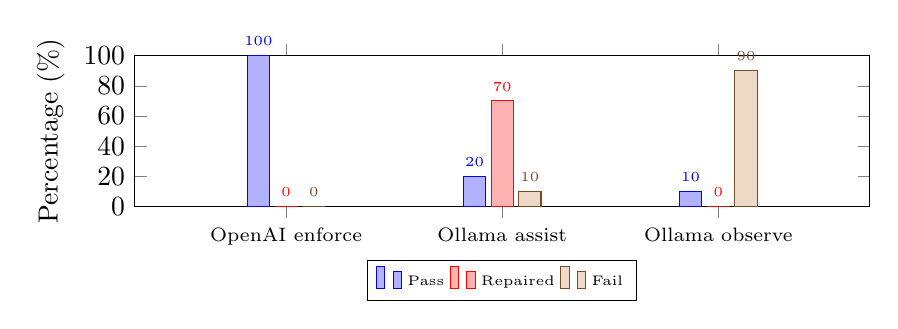
\begin{tikzpicture}
\begin{axis}[
  ybar,
  symbolic x coords={OpenAI enforce, Ollama assist, Ollama observe},
  xtick=data,
  xticklabel style={font=\scriptsize, align=center},
  ylabel={Percentage (\%)},
  ymin=0, ymax=100,
  legend style={at={(0.5,-0.35)}, anchor=north, legend columns=3, font=\tiny},
  width=0.9\columnwidth,
  height=3.5cm,
  bar width=8pt,
  enlarge x limits=0.35,
  nodes near coords,
  every node near coord/.append style={font=\tiny}
]
\addplot coordinates {(OpenAI enforce,100) (Ollama assist,20) (Ollama observe,10)};
\addplot coordinates {(OpenAI enforce,0) (Ollama assist,70) (Ollama observe,0)};
\addplot coordinates {(OpenAI enforce,0) (Ollama assist,10) (Ollama observe,90)};
\legend{Pass, Repaired, Fail}
\end{axis}
\end{tikzpicture}
\caption{Validation Outcomes by Configuration}
\label{fig:results}
\end{figure}

\textbf{OpenAI (enforce)}: 100\% first-attempt success, 847ms mean latency (\(\sigma\)=124), consistent with benchmarks~\cite{achiam2023gpt}. \textbf{Ollama (assist)}: 90\% total success (20\% pass + 70\% repair). Repairs: enum lowercasing (86\%), fence stripping (14\%). One failure: nested structure vs. flat schema. Latency: 2,314ms (\(\sigma\)=418) on M1 MacBook Pro 16GB. \textbf{Ollama (observe, no-validation baseline)}: 10\% success, establishing the critical value of constraint augmentation. Differences between enforce and assist are statistically significant (Welch's t-test, \(p < 0.05\), \(n = 10\)).

\subsection{Ablation Study}

\begin{table}[H]
\centering
\caption{Auto-Repair Impact}
\label{tab:ablation}
\scriptsize
\begin{tabular}{@{}lcc@{}}
\toprule
\textbf{Configuration} & \textbf{Success} & \textbf{Primary Failure} \\
\midrule
Assist + Repair & 90\% & Structural \\
Assist (no repair) & 30\% & Casing/fences \\
Observe (baseline) & 10\% & Multiple \\
\bottomrule
\end{tabular}
\end{table}

Disabling repair reduced success from 90\% to 30\%, demonstrating repair bridges model behavior and contract expectations.

\subsection{Reproducibility and CI/CD}

JUnit output enables standard test aggregation. Artifact saving (\texttt{--save-io}) generates audit trails: \texttt{input\_final.txt}, \texttt{output\_raw.txt}, \texttt{output\_norm.txt}, \texttt{run.json} with metadata (mode, status, checks, ledger, timestamp) per ISO 29119 traceability requirements~\cite{iso29119}. Validation overhead: \(<\)5ms per fixture.

\section{Discussion}

\subsection{Scientific Limitations}

PCSL v0.1 addresses structural validation (syntax, required fields, enums) but provides limited semantic validation. Check expressiveness is bounded by deterministic predicates; semantic correctness (e.g., correct classification logic) requires higher-order validation (e.g., LLM-as-a-judge~\cite{zheng2023judging}). Provider non-determinism remains fundamental: syntactically valid outputs may be semantically incorrect. Tolerance thresholds \(\tau\) require domain-specific calibration—no universal value exists.

\subsection{Practical Limitations}

Focus on JSON outputs limits applicability to free-text, dialogue, and multimodal generation. Current adapters (OpenAI, Ollama) require manual integration; plugin architecture would enable community contributions. Auto-repair effectiveness (90\%) risks masking genuine model issues; repair rate monitoring is essential for production systems.

\subsection{Compliance as Audit Layer}

The EU AI Act~\cite{euaiact2024} mandates transparency, auditability, and risk management for high-risk AI systems. PCSL operationalizes compliance-as-code for AI systems, providing machine-verifiable contracts, auditable traces, and CI/CD gating aligned with ISO/IEC/IEEE testing principles and the EU AI Act's documentation requirements. By aligning with ISO/IEC/IEEE 29119 testing standards~\cite{iso29119}, PCSL facilitates integration into existing quality assurance processes for regulated industries (healthcare, finance, legal services).

PCSL serves as a proto-standard for LLM specification, analogous to OpenAPI for REST, facilitating cross-organizational prompt sharing and regulatory compliance documentation.

\subsection{Future Work}

\begin{table}[H]
\centering
\caption{PCSL Roadmap}
\label{tab:roadmap}
\scriptsize
\begin{tabular}{@{}llp{4.5cm}@{}}
\toprule
\textbf{Version} & \textbf{Target} & \textbf{Goals} \\
\midrule
v0.2 & Q2 2025 & Plugin architecture, Anthropic/Cohere adapters \\
v0.3 & Q3 2025 & Semantic checks (similarity, sentiment, toxicity), LLM-judge, flexible parsing (YAML, XML) \\
v1.0 & Q1 2026 & Multi-turn contracts, differential testing, contract synthesis, standardization proposal \\
\bottomrule
\end{tabular}
\end{table}

Open problems: (1) differential testing for model drift, (2) adaptive validation thresholds via learned metrics, (3) causal validation, (4) multi-turn dialogue contracts, (5) adversarial generation, (6) contract synthesis from examples.

\section{Conclusion}

This paper introduced PCSL, the first formal specification language for LLM prompt testing. Through mathematical formalization extending design-by-contract to probabilistic systems and provider-agnostic execution, PCSL addresses critical gaps in reproducibility, reliability, and regulatory compliance. Evaluation demonstrated 100\% validation success with schema enforcement and 90\% with constraint augmentation (vs. 10\% no-validation baseline), validating capability negotiation and auto-repair mechanisms with statistical significance (\(p < 0.05\)).

PCSL introduces "type safety" for prompt engineering: declarative, machine-verifiable contracts enabling systematic testing, CI/CD integration per ISO 29119~\cite{iso29119}, and compliance auditing per EU AI Act~\cite{euaiact2024}. As LLMs integrate into critical systems, formal validation becomes essential. PCSL provides a foundation toward a universal contract standard for human-AI interaction. The framework is open source at \url{https://github.com/philippmelikidis/prompt-contracts}.

\bibliographystyle{ACM-Reference-Format}
\bibliography{references}

\end{document}
